

\chapter{Introducción específica} % Main chapter title

\label{Chapter2}

%----------------------------------------------------------------------------------------
%	SECTION 1
%----------------------------------------------------------------------------------------
Esta sección presenta una breve introducción técnica a las herramientas hardware y software utilizadas en el trabajo.

\section{Tecnologías de hardware utilizadas}

\subsection{Espressif ESP32}


ESP32 \cite{ESP32} es una serie de microcontroladores embebidos en un chip con Wi-Fi y Bluetooth integrados, de bajo costo y consumo, desarrollado por \textit{Espressif Systems}. Emplea dos cores Xtensa® 32-bit LX6 CPU, incluye interruptores de antena, amplificador de potencia, amplificador de recepción de bajo ruido, un co-procesador ULP (Ultra Low Power), módulos de administración de energía y varios periféricos.
En la siguiente imagen (\ref{fig:esp32}) se puede apreciar la placa ESP32-WROOM-32D \cite{ESP32_wroom_32d_datasheet} utilizada para el desarrollo del presente trabajo.

\begin{figure}[h]
    \centering
    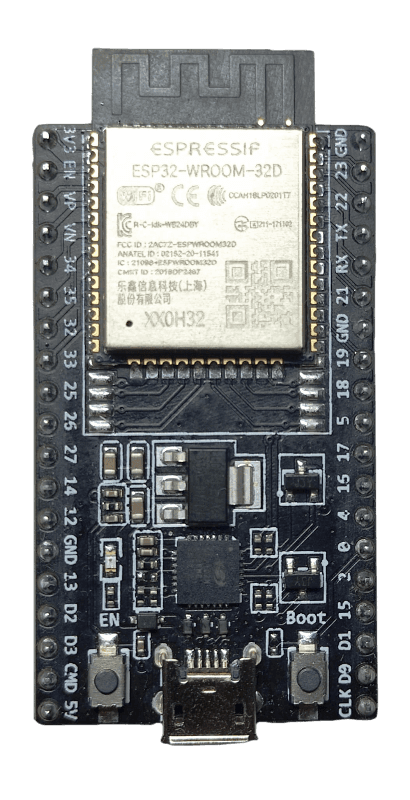
\includegraphics[scale=0.15]{esp32_2}
    \caption{Microcontrolador ESP32-WROOM-32D.}
    \label{fig:esp32}
\end{figure}


\subsection{Sensor de temperatura y humedad DHT11}

El DHT11 \cite{DHT11_datasheet} es un sensor digital de temperatura y humedad relativa de bajo costo y fácil uso. Integra un sensor capacitivo de humedad y un termistor para medir el aire circundante, y muestra los datos mediante una señal digital en el pin de datos (no posee salida analógica). Entre otras aplicaciones se lo suele utilizar principalmente en aplicaciones relacionadas al control automático de temperatura, aire acondicionado y monitoreo ambiental en agricultura. En la figura \ref{fig:dht11} se puede apreciar una imagen del componente.

\begin{figure}[h]
    \centering
    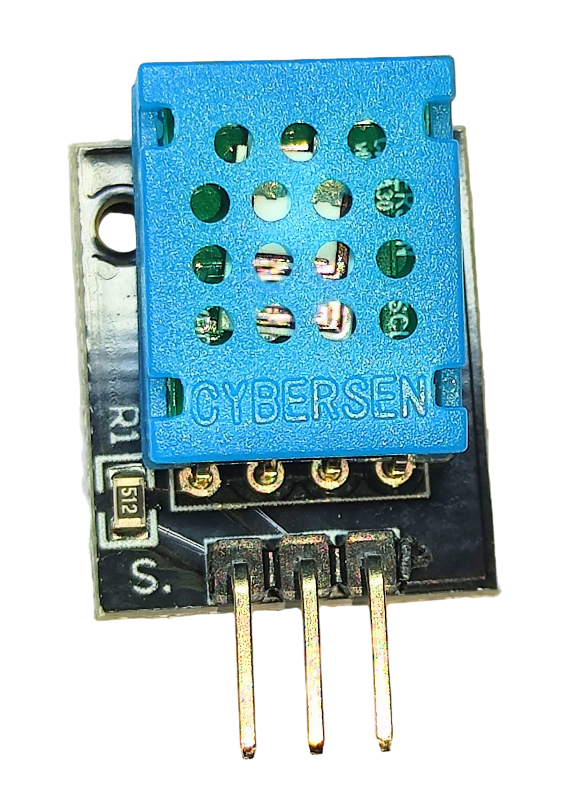
\includegraphics[scale=0.1]{dht11_2}
    \caption{Sensor DHT11.}
    \label{fig:dht11}
\end{figure}

\subsection{Sensor de presión BMP280}

El BMP280 \cite{BMP280_datasheet} es un sensor de presión barométrica absoluta, especialmente factible para aplicaciones móviles que puede ser utilizado con I2C o SPI. Permite alta precisión y linealidad, estabilidad a largo plazo, alta robustez a un muy bajo consumo. En la figura \ref{fig:bmp280} se puede apreciar una imagen del componente.

\begin{figure}[h]
    \centering
    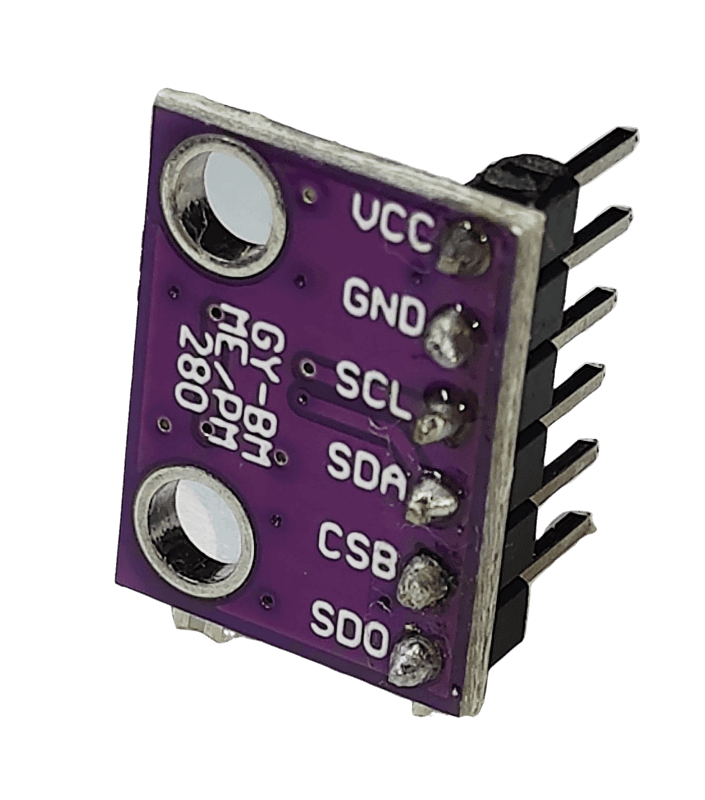
\includegraphics[scale=0.10]{bmp280_2}
    \caption{Sensor BMP280.}
    \label{fig:bmp280}
\end{figure}

\subsection{Fotoresistor como sensor de luminosidad}

El fotoresistor es una resistencia eléctrica que varía su valor en función de la cantidad de luz que incide sobre su superficie. 
Cuando el fotoresistor no está expuesto a radiaciones luminosas, los electrones están firmemente unidos en los átomos que lo conforman, por lo que alcanza su máxima resistencia eléctrica, y cuando sobre él inciden radiaciones luminosas, esta energía libera los electrones con lo cual el material se vuelve más conductor, y se disminuye su resistencia. En la figura \ref{fig:fotoresistor} se puede apreciar una imagen del componente.

\begin{figure}[h]
    \centering
    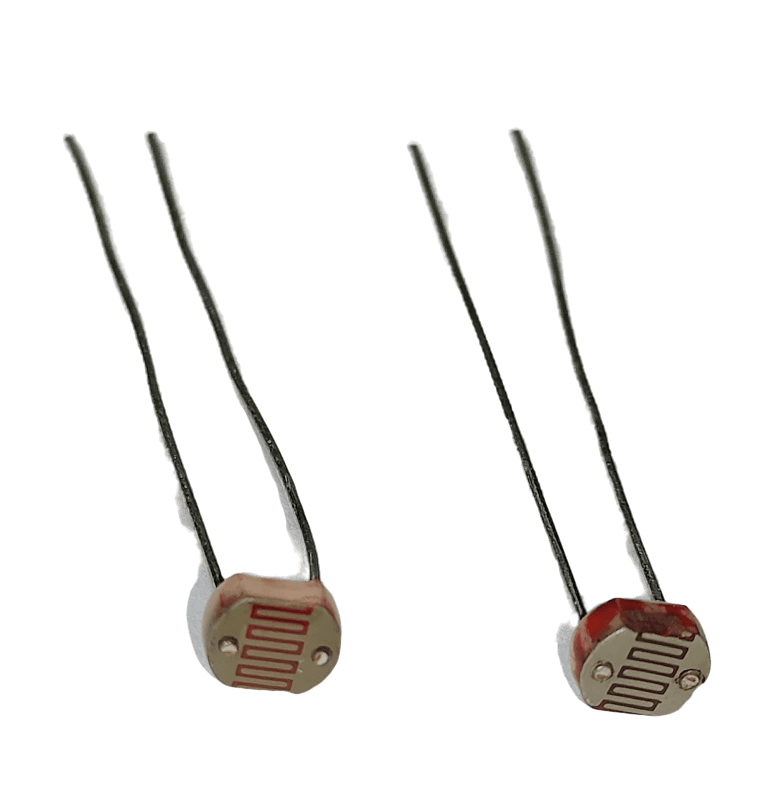
\includegraphics[scale=0.2]{fot2}
    \caption{Fotoresistor.}
    \label{fig:fotoresistor}
\end{figure}

\subsection{Joystick analógico}
 
El módulo de joystick analógico \cite{analog_joystick_datasheet} está construido sobre el montaje de dos potenciómetros en un ángulo de 90 grados. Los potenciómetros están conectados a una palanca corta centrada por resortes. 
Este módulo produce una salida de alrededor de 2,5 Volts cuando la palanca se encuentra en reposo (en el centro), mientras que al desplazarse hará que la salida varíe de 0 a 5 Volts dependiendo de su posición. La obtención de los valores en Volts se obtiene tras convertir las lecturas en niveles lógicos mediante el módulo ADC (conversor analógico digital) \cite{ESP32_adc} del microcontrolador ESP32. En la figura \ref{fig:joystick} se puede apreciar una imagen del componente.

\begin{figure}[h]
    \centering
    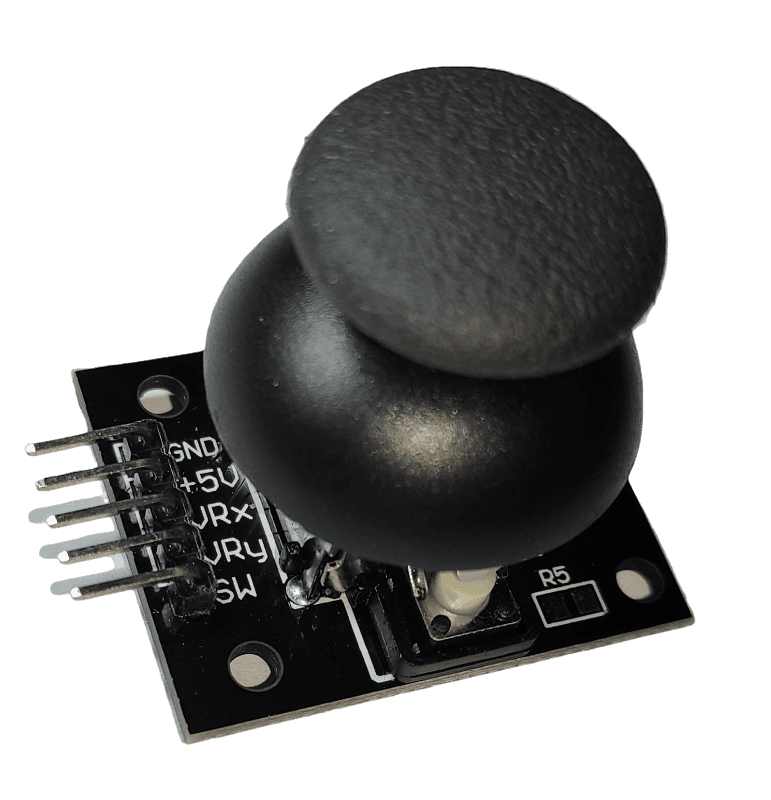
\includegraphics[scale=0.10]{joystick2}
    \caption{Joystick analógico.}
    \label{fig:joystick}
\end{figure}


\subsection{Display LCM1602A}
El display LCM1602A \cite{LCM1602A_datasheet} consta de una pantalla de cristal líquido que permite representar dos filas con hasta 16 caracteres alfanuméricos en cada una y dado que se encuentra integrada a una interfaz adaptadora I2C puede ser controlada por este protocolo. En la figura \ref{fig:display} se puede apreciar una imagen del componente.

\begin{figure}[h]
    \centering
    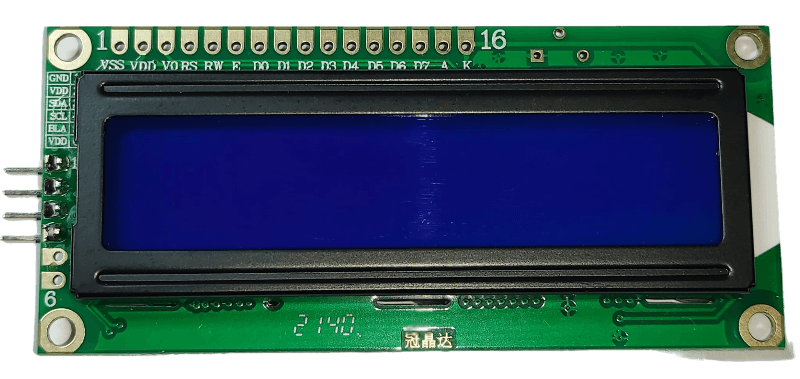
\includegraphics[scale=0.20]{display2}
    \caption{Display LCM1602A.}
    \label{fig:display}
\end{figure}

\subsection{Motores de corriente continua}
El motor DC (corriente continua) \cite{dc_motor_datasheet} es un electromotor que transforma energía eléctrica en energía mecánica. Estos motores operan con un voltaje entre 3 y 6 Volts, corriente de 150 mA, permiten una velocidad de entre 90 y 200 RPM y un torque de entre 0,15 Nm y 0,60 Nm. En la figura \ref{fig:dc_motors} se puede apreciar una imagen del componente.


%\begin{figure}[htbp]
%\centering
\begin{center}
  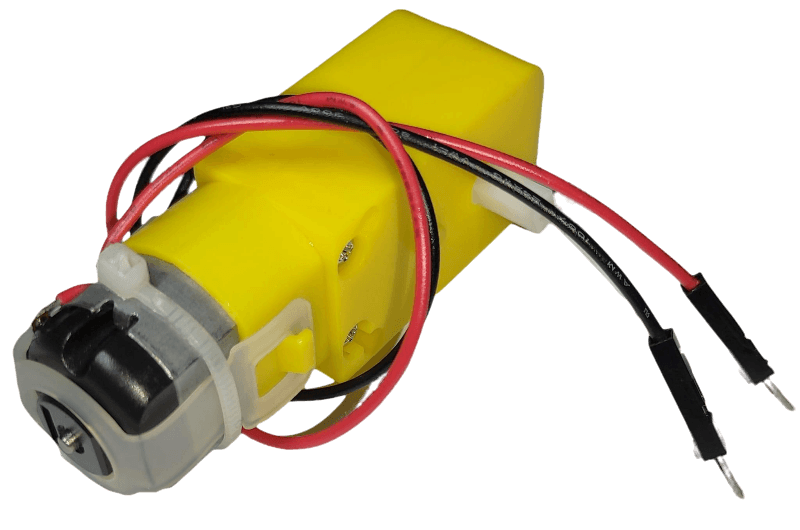
\includegraphics[scale=0.13]{engine2}
    \captionof{figure}{Motor de corriente continua.}
    \label{fig:dc_motors}
\end{center}
  
%\end{figure}



\section{Tecnologías de software utilizadas} 

\subsection{Marco de trabajo ESP-IDF}

\textit{Espressif Systems} proporciona recursos básicos de hardware y software para ayudar a los desarrolladores de aplicaciones a realizar sus ideas utilizando el hardware de la serie ESP32. El framework de software de Espressif está destinado al desarrollo de aplicaciones de IoT (Internet de las cosas) con Wi-Fi, Bluetooth, administración de energía y varias otras características del sistema.
Sus componentes son:
\begin{enumerate}
	\item Toolchain, utilizado para compilar el código para ESP32.
	\item Build tools, que provee utilidades como CMake \cite{cmake_website} y Ninja \cite{ninja_website} para construir la aplicación completa para ESP32.
	\item ESP-IDF \cite{ESPIDF_home}, que brinda la API de desarrollo para ESP32 y scripts para ejecutar Toolchain.
	
\end{enumerate}

Además de las herramientas mencionadas se utilizó el conjunto de bibliotecas y drivers provistos por el proyecto ESP-IDF-Lib \cite{esp_idf_lib_website} basados en el framework ESP-IDF.

En la figura \ref{fig:esp-idf} se puede apreciar una imagen del proceso de desarrollo y despliegue usando el framework ESP-IDF.

\begin{figure}[h]
    \centering
    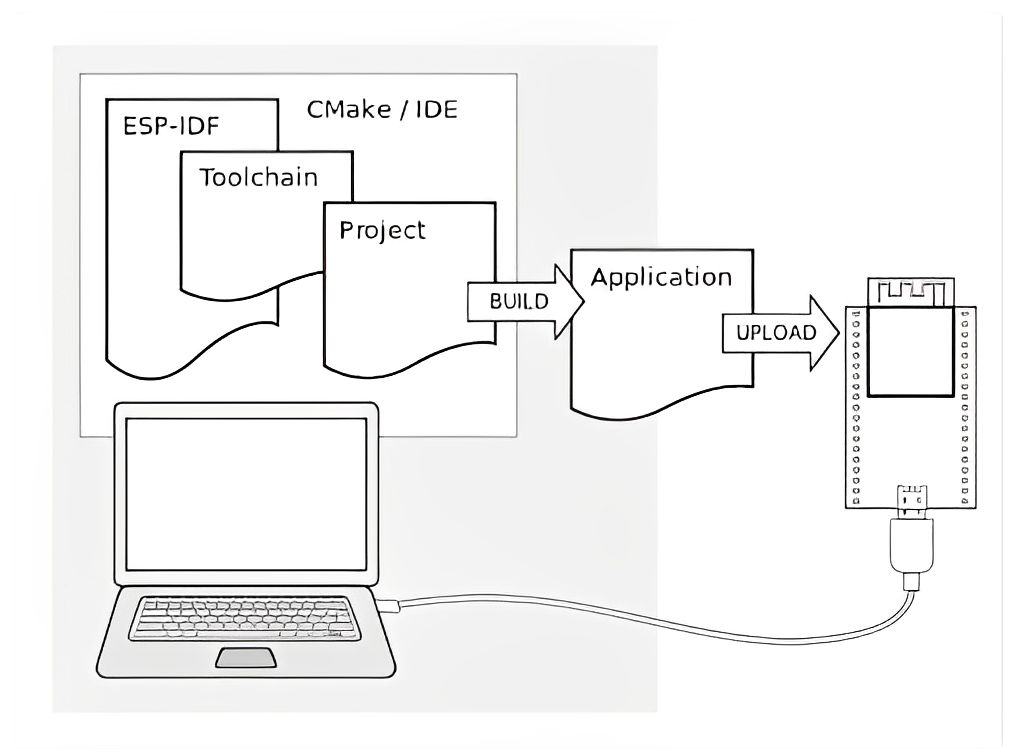
\includegraphics[scale=0.25]{esp-idf-2}
    \caption{Proceso de desarrollo utilizando ESP-IDF\protect\footnotemark.}
    \label{fig:esp-idf}
\end{figure}

%\begin{center}
%\end{center}
%
\includegraphics[scale=0.25]{espressif}

\footnotetext{Imagen tomada de \cite{espressif-website-esp-idf}}

\subsection{Plataforma Docker}

Docker \cite{docker_website} es un proyecto de código abierto que automatiza el despliegue de aplicaciones dentro de contenedores de software, proporcionando una capa adicional de abstracción y automatización de virtualización de aplicaciones en múltiples sistemas operativos.​ Docker utiliza características de aislamiento de recursos del kernel Linux, tales como cgroups y espacios de nombres (namespaces) para permitir que contenedores livianos independientes se ejecuten en paralelo de manera aislada evitando la sobrecarga de iniciar y mantener máquinas virtuales.

%
\includegraphics[scale=0.15]{docker}

\subsection{Visual Studio Code}

Visual Studio Code \cite{vscode_website} es un editor de código fuente desarrollado por Microsoft para Windows, Linux, macOS y Web. Incluye soporte para la depuración, control integrado de Git, resaltado de sintaxis, finalización inteligente de código, fragmentos y refactorización de código. 

%
\includegraphics[scale=0.15]{vscode}

\subsection{Sistema operativo Ubuntu}
Ubuntu \cite{ubuntu_website} es una distribución Linux basada en Debian GNU/Linux y patrocinado por Canonical, que incluye principalmente software libre y de código abierto. Puede utilizarse en ordenadores y servidores, está orientado al usuario promedio, con un fuerte enfoque en la facilidad de uso y en mejorar la experiencia del usuario. 

%
\includegraphics[scale=0.25]{ubuntu}
